
\section{Results}

\par With our three models in hands, we turn to our questions of interest.

\bigskip \textbf{Question 1: How do changes in our variables affect the odds that an American adult believes in anthropogenic climate change?}

\par \bigskip We can answer this question by finding the odds ratio for each coefficient $\beta_k$, given by $e^{\beta_k}$, as well as the upper and lower bounds of its 95 percent confidence interval, given by $e^{\beta_k \pm z_{.025} {SE_{\beta_k}}}$ where $z_{.025}$ is the  quantile $q$ of the standard normal distribution for which $P(x < q) = .025$. Results are listed in Figure \ref{fig:oddsratio_tables}. For examples of how to interpret these numbers, consider the odds ratios for $Age$ and $ScientistsGood$ in Model 1. We estimate that an American adult is 0.971 times less likely to believe in climate change for every year they have been alive, and are 95 percent confident that the true shrinkage factor is between 0.954 and 0.988. We also estimate that an American adult who believes scientists are generally honest and serve the public good is 3.589 times more likely to believe in anthropogenic climate change than an American adult who does not, and we are 95 percent confidence that the true growth factor is between 2.429 and 5.302.

\begin{figure}[h]
    \centering
    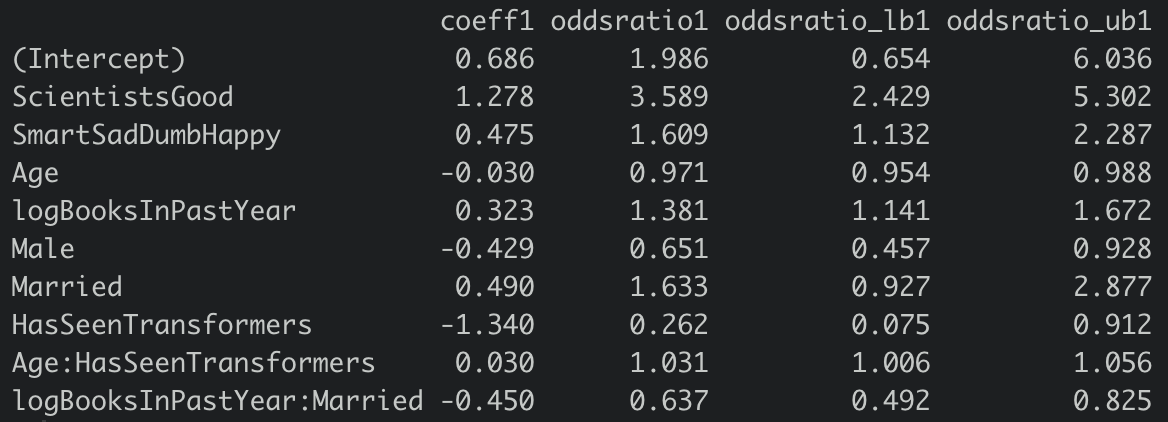
\includegraphics[scale=.5]{oddsratios_1.png}\vspace{.2in}
    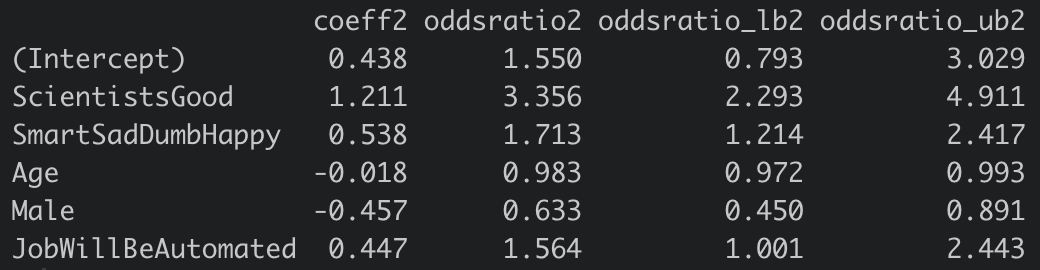
\includegraphics[scale=.5]{oddsratios_2.png}\vspace{.2in}
    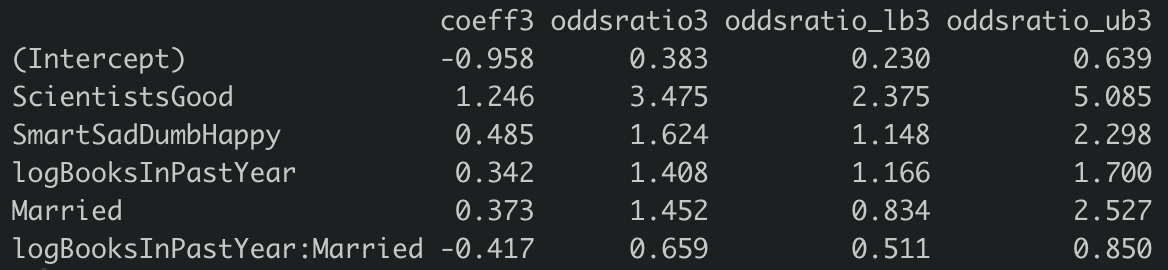
\includegraphics[scale=.5]{oddsratios_3.png}
    \caption{Tables of the estimated odds ratios for our model coefficients, with associated 95 percent confidence intervals}
    \label{fig:oddsratio_tables}
\end{figure}

\newpage

\bigskip \textbf{Question 2: How accurately can our model predict the likelihood that various profiles of American adults believe in anthropogenic climate change?}

\par \bigskip We answered this question in its grandest sense with our training models in the previous section. With accuracy proportions of 0.697 for Model 1, 0.686 for Model 2, and 0.699 for Model 3, all three models turn out to have decent accuracy with pure up-or-down predictions. For the sake of illustration, we use the full models to generate probabilities for a handful of respondent profiles, the results of which are shown in Figure \ref{fig:predictions}. Based on the signs on each coefficient, the first row is designed to represent someone who is very likely to believe in climate change, and the second row someone who is very unlikely to believe in climate change. The third row contains answers provided by a friend of the author.

\begin{figure}[h]
    \centering
    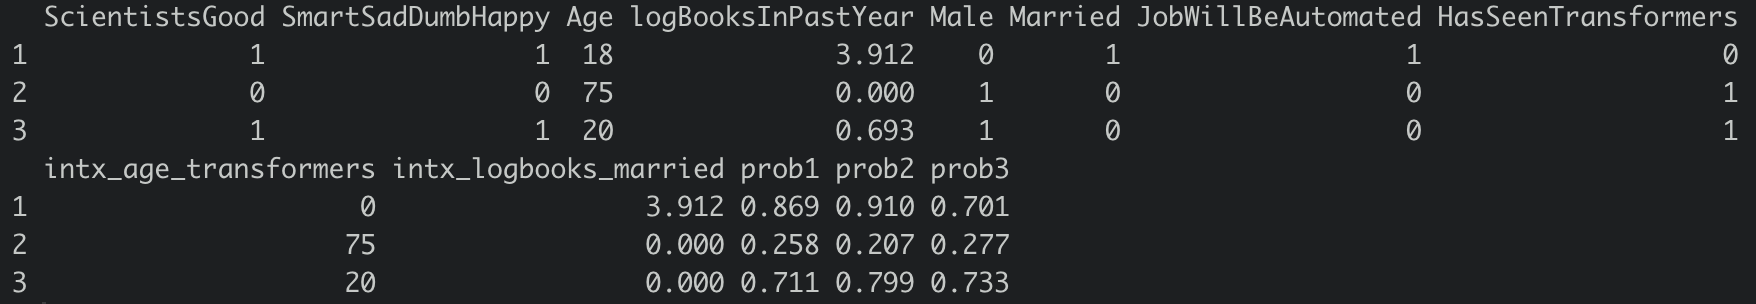
\includegraphics[scale=.5]{predictions.png}
    \caption{Model predictions for three profiles of American adults}
    \label{fig:predictions}
\end{figure}

\par We see that, of the three models, Model 1 returns the highest probability for our likely believer and the lowest for our unlikely believer. In contrast, Model 3 gives the most conservative predictions for those cases. This is probably because Model 1 has the most predictors and we stacked the deck in favor of climate change belief as much as possible, while Model 3 has the fewest. If the reader wants more aggressive predictions, they should use Model 1; for more cautious predictions, Model 3 is best.

\par \bigskip Each of our models correctly predicted with moderate certainty that the author's friend believes in climate change. Interestingly, his first three answers were consistent with the believer, while the other five were consistent with the nonbeliever, and yet he was predicted to believe in climate change. This emphasizes the outsized contributions of $ScientistsGood$ and $Age$ to our model.

\newpage

\subsection{Further Discussion}

\par Clearly, our inferences are limited to the population of American adults. These models should not be used at times far from the year 2017, either. While we can probably expect our variables to remain somewhat constant over a few years, the dynamics of belief in climate change among the public were very likely different 5-10 years before this survey. Even four years later, we would want to use a survey conducted more recently to make conclusions about climate change belief in 2021.

\par \bigskip The reader should also keep in mind that our model conditions are not as robust as we would like them to be, and there are likely some relationships between the variables that artificially reinforce predictions. Recall that Model 2 appears to be the least collinear of the three, and Model 3 is the simplest. The cautious statistician should prefer these two models to Model 1, even though its variables offer more chances to differentiate between individuals.

\subsection{Conclusion}

\par In this paper, we sought to develop a logistic regression model for the probability that an American adult believes in human-caused climate change. Using three versions of stepwise regression, we found three suitable models, each with benefits and downsides. We then used our models to derive meaningful statistical statements about how our variables affect the odds of climate change belief.

\par \bigskip Note that the coefficient on $ScientistsGood$ is by far the largest in each of our models. Our study is observational and we cannot conclude whether trust in scientists causes greater climate change belief or vice versa, nor whether a third factor causes both. That said, it is worth exploring further how much the fostering of trust in scientists among the public can increase the number of adults who believe in climate change.